\documentclass[12pt,a4paper]{article}

% ==================================================
% 1. CONFIGURATION
% ==================================================

% Enable / disable title page
\newif\ifshowtitlepage
\showtitlepagetrue
% \showtitlepagefalse

% Document information
\newcommand{\worktitle}{Multi-State Choreography Design}
\newcommand{\worksubtitle}{NAO Robot Exercise System}
\newcommand{\teamname}{NAOMI}
\newcommand{\subject}{NAO Robot Exercise System}

\newcommand{\university}{Slovak University of Technology in Bratislava}
\newcommand{\faculty}{Faculty of Informatics and Information Technologies}

\newcommand{\academicyear}{2026/2027}
\newcommand{\location}{Bratislava}
\newcommand{\documentyear}{2026/2027}

% Team leaders
\newcommand{\leaderone}{Ing. Jakub Perdek, PhD.}
\newcommand{\leadertwo}{ doc. Ing. Fedor Lehocki PhD.}

% Team members
\newcommand{\memberone}{Bc. Akhmadinurov Amal}
\newcommand{\membertwo}{Bc. Danilov Denis}
\newcommand{\memberthree}{Bc. Dmitriev Anton}
\newcommand{\memberfour}{Bc. Gainetdinov Ruslan}
\newcommand{\memberfive}{Bc. Kuzin Timofei}
\newcommand{\membersix}{Bc. Tikhoblazhenko Alena}
\newcommand{\memberseven}{Bc. Zimnitski Aliaksei}


% ==================================================
% 2. PACKAGES
% ==================================================

\usepackage[
    a4paper,
    top=3cm,
    bottom=2.7cm,
    left=2.8cm,
    right=2.8cm,
    headheight=45pt,
    headsep=20pt
]{geometry}

\usepackage[T1]{fontenc}
\usepackage[utf8]{inputenc}
\usepackage[english]{babel}
\usepackage{lmodern}

\usepackage{graphicx}
\graphicspath{{../../assets/}{assets/}}
\usepackage{tikz}
\usetikzlibrary{arrows.meta,positioning}
\usepackage{listings}
\usepackage{enumitem}
\setlist[itemize]{itemsep=1pt,parsep=0pt,topsep=2pt}
\lstset{basicstyle=\ttfamily\scriptsize,breaklines=true,frame=single,columns=fullflexible,keepspaces=true}
\usepackage[table]{xcolor}
\usepackage{fancyhdr}
\usepackage{titlesec}
\usepackage{setspace}
\usepackage{lastpage}
\usepackage{array}
\usepackage{float}
\usepackage{caption}
\usepackage{booktabs}
\usepackage{tabularx}
\usepackage{lipsum}
\usepackage{csquotes}

% Hyperlinks
\usepackage[hidelinks]{hyperref}


% ==================================================
% 3. COLORS
% ==================================================

\definecolor{primary}{HTML}{000000}
\definecolor{secondary}{HTML}{000000}
\definecolor{muted}{HTML}{000000}
\definecolor{linecolor}{HTML}{000000}
\definecolor{naomiTableHeader}{HTML}{17445A}
\definecolor{naomiTableStripe}{HTML}{EDF7FA}
\definecolor{naomiTableRule}{HTML}{66BBD0}

% Ragged-right columns keep narrow table cells readable.
\newcolumntype{L}[1]{>{\raggedright\arraybackslash}p{#1}}
\newcolumntype{Y}{>{\raggedright\arraybackslash}X}


% ==================================================
% 4. TYPOGRAPHY
% ==================================================

\setstretch{1.2}

\setlength{\parindent}{0pt}
\setlength{\parskip}{7pt}

% Section
\titleformat{\section}
    {\Large\bfseries\color{primary}}
    {\thesection}
    {0.8em}
    {}

% Subsection
\titleformat{\subsection}
    {\large\bfseries\color{primary}}
    {\thesubsection}
    {0.8em}
    {}

% Subsubsection
\titleformat{\subsubsection}
    {\normalsize\bfseries\color{primary}}
    {\thesubsubsection}
    {0.8em}
    {}

\titlespacing*{\section}{0pt}{20pt}{10pt}
\titlespacing*{\subsection}{0pt}{14pt}{7pt}
\titlespacing*{\subsubsection}{0pt}{12pt}{5pt}

% Captions
\captionsetup{
    font=small,
    labelfont=bf,
    justification=centering
}

% ==================================================
% 5. HEADER AND FOOTER
% ==================================================

\pagestyle{fancy}
\fancyhf{}

% Header logo
\fancyhead[L]{
    
\includegraphics[
        width=4cm,
        height=1.15cm,
        keepaspectratio
    ]{horizontal.png}
}

% Header information
\fancyhead[R]{
    \begin{tabular}{r}
        {\footnotesize\bfseries \worksubtitle}\\[3pt]
        {\scriptsize Academic Year \academicyear}
    \end{tabular}
}

% Header line
\renewcommand{\headrulewidth}{0.7pt}

% Footer left
\fancyfoot[L]{
    {\scriptsize
    \teamname\enspace|\enspace\subject}
}

% Footer right
\fancyfoot[R]{
    {\scriptsize
    \thepage\enspace/\enspace\pageref{LastPage}}
}

% Footer line
\renewcommand{\footrulewidth}{0.4pt}

% Plain pages
\fancypagestyle{plain}{
    \fancyhf{}

    \fancyhead[L]{
        
\includegraphics[
            width=4cm,
            height=1.15cm,
            keepaspectratio
        ]{horizontal.png}
    }

    \fancyhead[R]{
        \begin{tabular}{r}
            {\footnotesize\bfseries \worksubtitle}\\[3pt]
            {\scriptsize Academic Year \academicyear}
        \end{tabular}
    }

    \fancyfoot[L]{
        {\scriptsize
        \teamname\enspace|\enspace\subject}
    }

    \fancyfoot[R]{
        {\scriptsize
        \thepage\enspace/\enspace\pageref{LastPage}}
    }

    \renewcommand{\headrulewidth}{0.7pt}
    \renewcommand{\footrulewidth}{0.4pt}
}




% ==================================================
% 6. TITLE PAGE
% ==================================================

\newcommand{\makemytitlepage}{
    \begin{titlepage}
        \thispagestyle{empty}
        \centering

        % ==========================================
        % UNIVERSITY LOGO
        % ==========================================

        \vspace*{0.3cm}

        
\includegraphics[
            width=6cm,
            height=5cm,
            keepaspectratio
        ]{vertical.png}

        \vspace{0.5cm}

        {\large\bfseries
        \university\par}

        \vspace{0.2cm}

        {\normalsize
        \faculty\par}

        % ==========================================
        % PROJECT TITLE
        % ==========================================

        \vspace{1.7cm}

        {\small\MakeUppercase{\worksubtitle}\par}

        \vspace{0.5cm}

        \begin{minipage}{0.95\textwidth}
            \centering

            {\fontsize{25}{32}\selectfont\bfseries
            \worktitle\par}
        \end{minipage}

        % ==========================================
        % TEAM INFORMATION
        % ==========================================

        \vfill

        \begin{minipage}{0.9\textwidth}
            \centering
            \begin{minipage}[t]{0.46\linewidth}
                \centering
                {\normalsize\bfseries Team Leaders\par}
                \vspace{0.25cm}
                {\small
                \leaderone\par
                \leadertwo\par}
            \end{minipage}%
            \hfill
            \begin{minipage}[t]{0.48\linewidth}
                \centering
                {\normalsize\bfseries Team Members\par}
                \vspace{0.25cm}
                {\small
                \memberone\par
                \membertwo\par
                \memberthree\par
                \memberfour\par
                \memberfive\par
                \membersix\par
                \memberseven\par}
            \end{minipage}
        \end{minipage}

        % ==========================================
        % BOTTOM INFORMATION
        % ==========================================

        \vfill

        {\small
        \location\enspace\textbullet\enspace\academicyear\par}

    \end{titlepage}
}

% ==================================================
% 7. IMAGE PLACEHOLDER
% ==================================================

% Usage:
% \imageplaceholder{Text}{Caption}

\newcommand{\imageplaceholder}[2]{

    \begin{figure}[H]
        \centering

        \begingroup
        \setlength{\fboxsep}{0pt}

        \fbox{
            \begin{minipage}[c][5cm][c]{0.85\textwidth}

                \centering

                {\Large\bfseries IMAGE}

                \vspace{0.3cm}

                {\normalsize #1}

            \end{minipage}
        }

        \endgroup

        \caption{#2}

    \end{figure}
}


% ==================================================
% 8. REAL IMAGE COMMAND
% ==================================================

% Usage:
% \documentimage{path}{caption}{label}

\newcommand{\documentimage}[3]{

    \begin{figure}[htbp]
        \centering

        \includegraphics[
            width=0.85\textwidth,
            keepaspectratio
        ]{#1}

        \caption{#2}
        \label{#3}

    \end{figure}
}


% ==================================================
% 9. TABLES
% ==================================================

% Usage:
% \begin{naomitable}{Caption}{label}
%     \begin{tabularx}{\textwidth}{L{2.8cm} Y L{2.6cm}}
%         \rowcolor{naomiTableHeader}
%         \textcolor{white}{\bfseries Name} & ... \\
%         ...
%         \arrayrulecolor{naomiTableRule}\bottomrule[1pt]
%     \end{tabularx}
% \end{naomitable}

\newenvironment{naomitable}[2]{%
    \begin{table}[H]
        \centering
        \caption{#1}
        \label{#2}
        \begingroup
        \small
        \renewcommand{\arraystretch}{1.4}
        \setlength{\tabcolsep}{7pt}
        \rowcolors{2}{naomiTableStripe}{white}
}{%
        \endgroup
    \end{table}
}

% Usage:
% \tableplaceholder{Caption}{label}

\newcommand{\tableplaceholder}[2]{
    \begin{naomitable}{#1}{#2}
        \begin{tabularx}{\textwidth}{L{2.8cm} Y L{2.6cm}}
            \rowcolor{naomiTableHeader}
            \textcolor{white}{\bfseries Name} &
            \textcolor{white}{\bfseries Description} &
            \textcolor{white}{\bfseries Status} \\
            Item A & Sample description & Completed \\
            Item B & Sample description & In Progress \\
            Item C & Sample description & Planned \\
            \arrayrulecolor{naomiTableRule}\bottomrule[1pt]
        \end{tabularx}
    \end{naomitable}
}


% ==================================================
% 10. DOCUMENT
% ==================================================

\begin{document}

\ifshowtitlepage
    \makemytitlepage
\fi

% ==================================================
% CONTEXT
% ==================================================

\section{Context and Requirements}

The supervisor requires multi-state choreographies. The design follows his
answers from November 2026:

\begin{itemize}
    \item A \textbf{state} is what the system currently calls an
          \emph{exercise}: frames converted from a video, voice lines, media
          and the number of repetitions. Each state is stored under its own
          hash. Existing exercises are therefore already valid states and
          need no migration.
    \item A \textbf{choreography} is a graph of states with transitions,
          stored at a higher level. It is created visually in the frontend.
    \item After performing a state, the application \textbf{waits for a
          state-change signal} sent through the API. No other logic is
          implemented, in particular no evaluation of the participant's
          movement.
    \item The API also allows \textbf{moving to a state without applying its
          content}, i.e.\ without robot movement and voice lines.
    \item States can be switched by pressing keys on a keyboard, as a simple
          client of the same API.
\end{itemize}

% ==================================================
% DATA MODEL
% ==================================================

\section{Data Model}

A choreography references existing exercises by their hash. Positions
\texttt{x} and \texttt{y} are used only by the graph editor.

\begin{lstlisting}
{
  "schema_version": 1,
  "id": "c1d2e3f4",
  "name": "Trening 1",
  "initial_state": "da48eac8",
  "states": [
    { "state_id": "da48eac8", "label": "Pohyb 1",        "x": 120, "y": 80  },
    { "state_id": "a3f9c1d2", "label": "Pohyb 2",        "x": 120, "y": 240 },
    { "state_id": "b7e2a091", "label": "Pohyb 2 oprava", "x": 320, "y": 320 }
  ],
  "transitions": [
    { "id": "t1", "from": "da48eac8", "to": "a3f9c1d2", "label": "Pohyb 1 hotovy" },
    { "id": "t2", "from": "a3f9c1d2", "to": "b7e2a091", "label": "Chyba 1" },
    { "id": "t3", "from": "b7e2a091", "to": "a3f9c1d2", "label": "Oprava 1 zrealizovana" }
  ]
}
\end{lstlisting}

\begin{figure}[H]
    \centering
    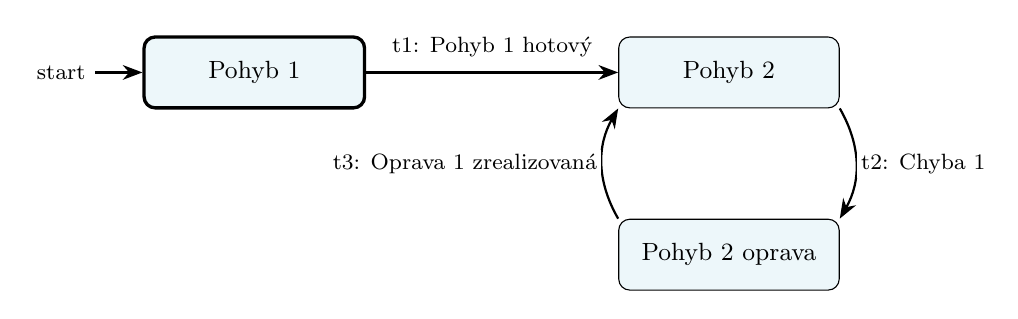
\begin{tikzpicture}[
        state/.style={draw, rounded corners, fill=naomiTableStripe,
                      minimum width=2.8cm, minimum height=0.9cm, font=\small},
        arr/.style={-{Stealth[length=2.5mm]}, thick},
        lbl/.style={font=\footnotesize, fill=white, inner sep=1.5pt}
    ]
        \node[state, very thick] (p1) {Pohyb 1};
        \node[state, right=3.2cm of p1] (p2) {Pohyb 2};
        \node[state, below=1.4cm of p2] (p2f) {Pohyb 2 oprava};
        \node[left=0.6cm of p1, font=\footnotesize] (start) {start};
        \draw[arr] (start) -- (p1);
        \draw[arr] (p1) -- node[font=\footnotesize, above=2pt] {t1: Pohyb 1 hotov\'y} (p2);
        \draw[arr] (p2.south east) to[bend left=30]
            node[lbl, right] {t2: Chyba 1} (p2f.north east);
        \draw[arr] (p2f.north west) to[bend left=30]
            node[lbl, left] {t3: Oprava 1 zrealizovan\'a} (p2.south west);
    \end{tikzpicture}
    \caption{The example choreography as a graph; the initial state has a thick border}
    \label{fig:graph}
\end{figure}

Validation rules: \texttt{initial\_state} is one of the states; every
transition connects two states of the same choreography; transition
identifiers are unique; every referenced state exists as an exercise.

Choreographies are stored as JSON files
\texttt{<id>.json} in the directory \texttt{\_choreographies} inside \texttt{EXERCISES\_DIR}. The listing of exercises
ignores this directory because it has no \texttt{config.json}, so existing
exercise endpoints keep working. All assets of a state (frames, media,
voice line sounds, source video) stay in the state's own directory.

% ==================================================
% API
% ==================================================

\section{API}

\subsection{Storing choreographies (exerciseConfigService, port 7001)}

\begin{naomitable}{Choreography endpoints}{tab:store}
    \begin{tabularx}{\textwidth}{L{1.6cm} L{5.4cm} Y}
        \rowcolor{naomiTableHeader}
        \textcolor{white}{\bfseries Method} &
        \textcolor{white}{\bfseries Path} &
        \textcolor{white}{\bfseries Purpose} \\
        GET    & \texttt{/choreography/list}      & list choreographies (id, name, number of states) \\
        POST   & \texttt{/choreography/create}    & create a choreography from a JSON document \\
        GET    & \texttt{/choreography/<id>}      & get the whole graph \\
        PUT    & \texttt{/choreography/<id>}      & replace the whole graph (sent by the editor) \\
        DELETE & \texttt{/choreography/<id>}      & delete the graph; the exercises stay \\
        \arrayrulecolor{naomiTableRule}\bottomrule[1pt]
    \end{tabularx}
\end{naomitable}

The editor always sends the whole graph, so there are no separate endpoints
for single states or transitions. An invalid graph is rejected with
\texttt{400} and a list of errors. Deleting an exercise that is used in a
choreography is rejected with \texttt{409}.

\subsection{Running choreographies (translator, port 7000)}

\begin{naomitable}{Run endpoints}{tab:run}
    \begin{tabularx}{\textwidth}{L{1.6cm} L{5.4cm} Y}
        \rowcolor{naomiTableHeader}
        \textcolor{white}{\bfseries Method} &
        \textcolor{white}{\bfseries Path} &
        \textcolor{white}{\bfseries Purpose} \\
        POST & \texttt{/choreography/<id>/run} & start a run and perform the initial state \\
        GET  & \texttt{/run/current}           & the active run, or \texttt{404} if none \\
        GET  & \texttt{/run/<run\_id>}         & current state, status and outgoing transitions \\
        POST & \texttt{/run/<run\_id>/signal}  & state-change signal: \texttt{\{"transition\_id": "t1"\}} \\
        POST & \texttt{/run/<run\_id>/goto}    & move to a state without applying its content: \texttt{\{"state\_id": "a3f9c1d2"\}} \\
        POST & \texttt{/run/<run\_id>/stop}    & stop the run \\
        \arrayrulecolor{naomiTableRule}\bottomrule[1pt]
    \end{tabularx}
\end{naomitable}

A run has the status \texttt{performing}, \texttt{waiting} or
\texttt{stopped}:

\begin{itemize}
    \item A state is performed in a background thread with the existing
          exercise logic (frames, voice lines, repetitions), so the API
          answers immediately and \texttt{stop} can interrupt the
          performance between frames.
    \item \texttt{signal} is accepted only in the status \texttt{waiting}
          and only for a transition that starts in the current state. The
          run moves to the target state and performs it. Otherwise the API
          answers \texttt{409} with the reason.
    \item \texttt{goto} is accepted in the status \texttt{waiting}, for any
          state of the choreography. It changes the current state without
          sending poses or voice lines; the run stays \texttt{waiting}.
    \item Only one run can be active, because there is one robot. Starting
          another run answers \texttt{409}.
    \item Runs are kept in memory; a restart of \texttt{translator} ends the
          active run.
\end{itemize}

% ==================================================
% RESPONSIBILITIES
% ==================================================

\section{Responsibilities of Services}

\begin{naomitable}{What each component owns}{tab:owners}
    \begin{tabularx}{\textwidth}{L{3.6cm} Y}
        \rowcolor{naomiTableHeader}
        \textcolor{white}{\bfseries Component} &
        \textcolor{white}{\bfseries Responsibility} \\
        exerciseConfigService & stores states (exercises) and choreographies, validates graphs \\
        translator            & runs choreographies, performs states, accepts signals; reuses the existing exercise run \\
        naoRobotAPI           & unchanged: moves the robot and says voice lines \\
        skeletonFinderAPI     & unchanged: converts videos to frames \\
        frontend              & creates and edits the graph (D3.js), shows the current state during a run, sends signals and \texttt{goto} on click \\
        keyboard client       & small script in \texttt{scripts/}; keys 1--9 send the outgoing transitions of the current state, \texttt{s} stops the run; no own logic \\
        \arrayrulecolor{naomiTableRule}\bottomrule[1pt]
    \end{tabularx}
\end{naomitable}

% ==================================================
% SCOPE
% ==================================================

\section{Scope for the Winter Semester}

\textbf{In scope:} storing choreographies, running them with signals and
\texttt{goto}, keyboard client, states created from one or more uploaded
videos, states with only a voice line or a robot command, creating the graph
and managing transitions in the frontend, schema and validation.

\textbf{Out of scope:} evaluation of the participant's movement and
automatic signals, authentication, application-specific states such as
``out of camera'' (users create them as ordinary states).

\textbf{Later extensions:} merging several videos into one state by
appending frames to the state's configuration (SCRUM-69), trimming videos
(SCRUM-70), a research application of choreographies in movement therapy
(SCRUM-102).

% ==================================================
% OPEN POINTS
% ==================================================

\section{Points to Confirm}

\begin{itemize}
    \item Choreographies are run by \texttt{translator} and stored by
          \texttt{exerciseConfigService}.
    \item A transition carries only a label; there are no conditions or
          repetition counters on transitions.
\end{itemize}

\end{document}